\begin{frame}[containsverbatim, t]{\inhibitglue Yes/Noチャート(異論は認める)}
  \sffamily
  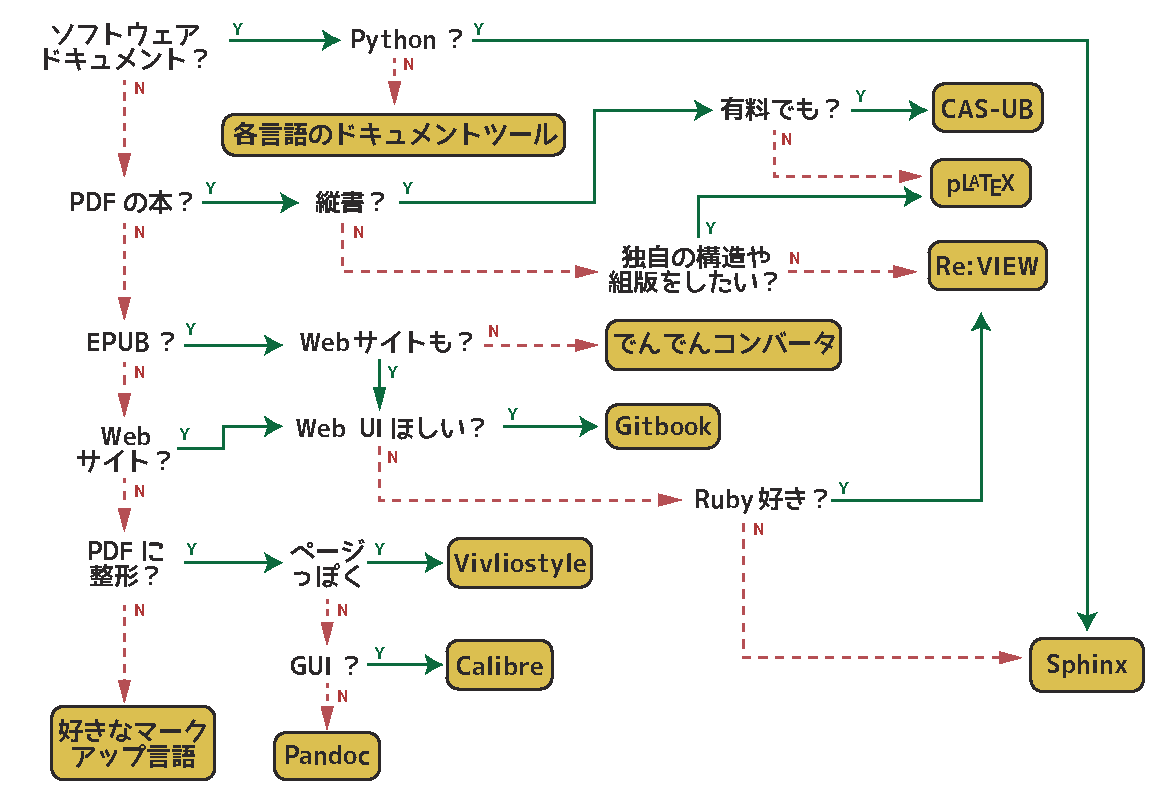
\includegraphics[width=.95\textwidth]{images/ynchart.pdf}
\end{frame}

\begin{frame}[containsverbatim, t]{\inhibitglue Sphinx}
  \sffamily
  
  \begin{itemize}
    \item ドキュメントをPDFでもEPUBでもHTMLでも出力したいといった用途に幅広く便利
    \item 特に、Pythonプログラムのドキュメントならこれ一択
    \item 構文などの拡張性は高い。既存の便利なエクステンションも豊富
    \item 紙書籍向けサポートは弱い
    \item \url{http://sphinx-doc.org/}(\url{http://sphinx-users.jp/})
  \end{itemize}

\end{frame}

\begin{frame}[containsverbatim, t]{\inhibitglue Re:VIEW}
  \sffamily
  
  \begin{itemize}
    \item 横書きの技術書(紙書籍向けPDF、電子書籍向けPDF、EPUB)が作りやすい
    \item 構文などの拡張性は高い
    \item 見た目をデフォルト以外にしたければ出力(LaTeX、CSS、InDesign)の知識が不可欠
    \item \url{https://github.com/kmuto/review/wiki}
  \end{itemize}

\end{frame}

%\begin{frame}[containsverbatim, t]{\inhibitglue EWB}
%  \sffamily
%  
%  \begin{itemize}
%    \item LaTeXっぽいシンタックスでテキストにレイアウト指示を入れる
%    \item アスキードワンゴで出版するなら、最有力
%  \end{itemize}
%
%\end{frame}

\begin{frame}[containsverbatim, t]{\inhibitglue Gitbook}
  \sffamily
  
  \begin{itemize}
    \item 技術書がGitHubとMarkdown(AsciiDomも可)で書ける。Web UIもある
    \item 構文の拡張性はないが、ある程度のスタイルは定義可能。いくつかプラグインもある
    \item PDF出力がひどい(CalibreのPDFエンジン)
    \item \url{https://www.gitbook.com}(\url{https://github.com/GitbookIO/gitbook})
  \end{itemize}

\end{frame}

\begin{frame}[containsverbatim, t]{\inhibitglue CAS-UB}
  \sffamily
  
  \begin{itemize}
    \item 縦書きを含む日本語の本(紙書籍向けPDF、電子書籍向けPDF、EPUB)が作れて、売れる
    \item 構文の拡張性はないが、ある程度のスタイルは定義可能
    \item Webブラウザでの編集が基本。1カ月の無償期間を超えると有償
    \item \url{http://www.cas-ub.com/index.php}
    \item (PressBooks、Booktype、Lean Book、Atlasなど、ほかにも同様の書籍執筆Webサービスはある)
  \end{itemize}

\end{frame}

%\begin{frame}[containsverbatim, t]{\inhibitglue PressBooks}
%  \sffamily
%  
%  \begin{itemize}
%    \item まともな本が作れて売れる
%    \item HTMLとCSSで書ける
%    \item PDFはPrinceで生成
%    \item Webブラウザでの編集が基本。課金しないと全ページに透かしが入る。日本語はNotoSans一択
%  \end{itemize}
%
%\end{frame}

%\begin{frame}[containsverbatim, t]{\inhibitglue Booktype}
%  \sffamily
%  
%  \begin{itemize}
%    \item 本が作れる。
%    \item HTMLとCSSで書ける
%    \item PDFはmPDF(PHPのネイティブなPDFエンジンであるFPDFの拡張)で生成
%    \item 日本語は文字化け
%  \end{itemize}
%
%\end{frame}
%
%\begin{frame}[containsverbatim, t]{\inhibitglue Atlas}
%  \sffamily
%  
%  \begin{itemize}
%    \item 米O'Reillyの著者用プラットフォーム
%    \item 入力はAsciiBooksとHTMLBooksで、出力はAH Formatterらしい
%    \item O'Reillyの著者にならないと使えない
%  \end{itemize}
%
%\end{frame}

\begin{frame}[containsverbatim, t]{\inhibitglue でんでんコンバーター}
  \sffamily
  
  \begin{itemize}
    \item 縦書きを含む日本語のEPUBが作れる
    \item 構文はMarkdownの独自拡張だが、HTMLの埋め込みはできる
    \item EPUBのみを生成するなら特に不満はないような?
    \item \url{http://conv.denshochan.com/}
  \end{itemize}

\end{frame}

%\begin{frame}[containsverbatim, t]{\inhibitglue BCCKS}
%  \sffamily
%  
%  \begin{itemize}
%    \item 縦書きを含め、まともな本(EPUBと紙)が作れて売れる
%    \item Wiki記法
%    \item 基本的にはEPUB出版用のサービスだが、オンデマンド用のPDF生成サービスがある
%    \item PDFがほしい場合には使えない
%  \end{itemize}
%
%\end{frame}


\begin{frame}[containsverbatim, t]{\inhibitglue Vivliostyle}
  \sffamily
  
  \begin{itemize}
    \item CSS組版エンジン
    \item Webブラウザで本のようなページが動的にレンダリングできる
    \item Webページ用のCSSからPDFが作れるわけではない
    \item \url{http://vivliostyle.com/ja/}
  \end{itemize}

\end{frame}

%\begin{frame}[containsverbatim, t]{\inhibitglue xml2tex}
%  \sffamily
%  
%  \begin{itemize}
%    \item XMLのシンタックスをLaTeXのシンタックスに対応づけるルールベース変換器
%    \item Gauche製
%    \item LaTeXに限らず、MarkdownやRe:VIEWフォーマットなどへの変換ルールも定義可能
%  \end{itemize}
%
%\end{frame}

\begin{frame}[containsverbatim, t]{\inhibitglue Pandoc}
  \sffamily
  
  \begin{itemize}
    \item さまざまなフォーマットを変換できる。似たようなツールはほかにもあるけど(kramdownとか)、対応フォーマット数が多く、しかも増えている
    \item Haskell製
    \item 基本的にはMarkdownを他の書式に変換するためのツールだと割り切ったほうが良い
    \item \url{http://pandoc.org/}
  \end{itemize}

\end{frame}

\begin{frame}[containsverbatim, t]{\inhibitglue Calibre}
  \sffamily
  
  \begin{itemize}
    \item 電子書籍の統合開発環境。なんでもできる。コマンド(\texttt{ebook-convert})もある
    \item Python製
    \item EPUB3には未対応
    \item \url{http://calibre-ebook.com/}
  \end{itemize}

\end{frame}

